% ============================================================
\chapter{Subdifferentials and Subgradients}
\label{ch:subdifferentials}
% ============================================================

\section{Introduction}

Here is a concrete problem: you want to minimise $\norm{x}_1$ subject to linear constraints---a central problem in sparse learning. But the $\ell_1$ norm is not differentiable at the origin: it has a ``corner.'' The gradient does not exist, and yet that is precisely where the minimum lies. How do you write an optimality condition without a gradient?

The answer, developed by Jean-Jacques Moreau and R.~Tyrrell Rockafellar in the 1960s, is the \emph{subdifferential}: instead of a single tangent plane, one considers \emph{all} hyperplanes that remain below the graph of the function. At points of differentiability, there is only one (the classical gradient). At corners, there are infinitely many, forming a convex compact set. This generalisation opens the door to a remarkably coherent theory of nonsmooth optimisation.

\begin{intuition}
For a differentiable function, the gradient defines the unique tangent hyperplane that
minorizes the function. For a nonsmooth convex function, there may exist \emph{multiple}
minorizing hyperplanes at a point --- their collection forms the subdifferential.
\end{intuition}

\section{Definition of Subgradient and Subdifferential}

\begin{definition}[Subgradient]
Let $f : \R^n \to \R \cup \{+\infty\}$ be a convex function. A vector $g \in \R^n$
is a \emph{subgradient} of $f$ at $x \in \mathrm{dom}(f)$ if:
\[
    f(y) \geq f(x) + \inner{g}{y - x}, \quad \forall y \in \R^n.
\]
\end{definition}

\begin{definition}[Subdifferential]
The \emph{subdifferential} of $f$ at $x$, denoted $\partial f(x)$, is the set of all
subgradients of $f$ at $x$:
\[
    \partial f(x) = \{g \in \R^n \mid f(y) \geq f(x) + \inner{g}{y-x}, \; \forall y \in \R^n\}.
\]
If $x \notin \mathrm{dom}(f)$, we set $\partial f(x) = \emptyset$.
\end{definition}

\begin{theorem}[Existence of Subgradients]
\label{thm:sg_existence}
Let $f : \R^n \to \R \cup \{+\infty\}$ be proper convex. Then
$\partial f(x) \neq \emptyset$ for all $x \in \mathrm{ri}(\mathrm{dom}(f))$.
In particular, if $\mathrm{dom}(f)$ is open, $\partial f(x) \neq \emptyset$ for all
$x \in \mathrm{dom}(f)$.
\end{theorem}

\begin{proof}
Let $x \in \mathrm{ri}(\mathrm{dom}(f))$. The point $(x, f(x))$ lies on the boundary
of $\mathrm{epi}(f)$, which is convex. By the supporting hyperplane theorem, there
exists $(g, -\alpha) \neq 0$ such that:
\[
    \inner{g}{y - x} - \alpha(t - f(x)) \leq 0, \quad \forall (y,t) \in \mathrm{epi}(f).
\]
Taking $y = x$ and $t \to +\infty$, we get $\alpha \geq 0$. If $\alpha = 0$, then
$\inner{g}{y-x} \leq 0$ for all $y \in \mathrm{dom}(f)$, contradicting
$x \in \mathrm{ri}(\mathrm{dom}(f))$ (unless $g = 0$). So $\alpha > 0$, and
$g/\alpha$ is a subgradient.
\end{proof}

\section{Properties of the Subdifferential}

\begin{theorem}[Fundamental Properties]
\label{thm:subdiff_props}
Let $f : \R^n \to \R \cup \{+\infty\}$ be proper convex.
\begin{enumerate}
    \item $\partial f(x)$ is a closed convex set (possibly empty).
    \item If $f$ is differentiable at $x$, then $\partial f(x) = \{\nabla f(x)\}$.
    \item $\partial f(x)$ is bounded if $x \in \mathrm{int}(\mathrm{dom}(f))$.
    \item $x^*$ minimizes $f$ if and only if $0 \in \partial f(x^*)$.
\end{enumerate}
\end{theorem}

\begin{proof}[Proof of (4)]
$(\Rightarrow)$ If $x^*$ minimizes $f$, then $f(y) \geq f(x^*)$ for all $y$, i.e.,
$f(y) \geq f(x^*) + \inner{0}{y - x^*}$, so $0 \in \partial f(x^*)$.

$(\Leftarrow)$ If $0 \in \partial f(x^*)$, then
$f(y) \geq f(x^*) + \inner{0}{y-x^*} = f(x^*)$ for all $y$, so $x^*$ is a global
minimizer.
\end{proof}

\begin{keyformulas}[title=\textbf{Subdifferential Optimality Condition}]
\[
    x^* \in \argmin_{x \in \R^n} f(x) \quad \Longleftrightarrow \quad 0 \in \partial f(x^*).
\]
This is the generalization of $\nabla f(x^*) = 0$ to the nonsmooth case.
\end{keyformulas}

\section{Examples of Subdifferentials}

\begin{example}[Absolute Value]
For $f(x) = \abs{x}$ on $\R$:
\[
    \partial f(x) = \begin{cases}
        \{-1\} & \text{if } x < 0, \\
        [-1, 1] & \text{if } x = 0, \\
        \{1\} & \text{if } x > 0.
    \end{cases}
\]
\end{example}

\begin{example}[$\ell_1$ Norm]
For $f(x) = \norm{x}_1 = \sum_i \abs{x_i}$ on $\R^n$:
\[
    \partial f(x) = \{g \in \R^n \mid g_i = \mathrm{sign}(x_i) \text{ if } x_i \neq 0, \;
    g_i \in [-1,1] \text{ if } x_i = 0\}.
\]
\end{example}

\begin{example}[Maximum of Smooth Functions]
For $f(x) = \max(f_1(x), \ldots, f_k(x))$ with $f_i$ differentiable and convex:
\[
    \partial f(x) = \mathrm{conv}\{\nabla f_i(x) \mid i \in I(x)\},
\]
where $I(x) = \{i \mid f_i(x) = f(x)\}$ is the set of active indices.
\end{example}

\begin{example}[Indicator Function]
For $f = \iota_C$ (indicator of a closed convex set $C$):
\[
    \partial \iota_C(x) = N_C(x) = \{g \in \R^n \mid \inner{g}{y-x} \leq 0, \; \forall y \in C\},
\]
which is the \emph{normal cone} to $C$ at $x$.
\end{example}

\section{Subdifferential Calculus Rules}

\begin{theorem}[Moreau--Rockafellar Sum Rule]
\label{thm:mr_sum}
Let $f_1, f_2 : \R^n \to \R \cup \{+\infty\}$ be proper convex. If
$\mathrm{ri}(\mathrm{dom}(f_1)) \cap \mathrm{ri}(\mathrm{dom}(f_2)) \neq \emptyset$,
then:
\[
    \partial(f_1 + f_2)(x) = \partial f_1(x) + \partial f_2(x).
\]
\end{theorem}

\begin{theorem}[Chain Rule]
\label{thm:chain}
Let $f$ be convex and $g(x) = f(Ax + b)$ with $A \in \R^{m \times n}$,
provided $Ax + b \in \mathrm{ri}(\mathrm{dom}(f))$. Then:
\[
    \partial g(x) = A^T \partial f(Ax + b).
\]
\end{theorem}

\begin{theorem}[Subdifferential of the Maximum]
Let $f_1, \ldots, f_k$ be convex. For $f(x) = \max_i f_i(x)$:
\[
    \partial f(x) = \mathrm{conv}\left(\bigcup_{i \in I(x)} \partial f_i(x)\right),
\]
where $I(x) = \{i \mid f_i(x) = f(x)\}$.
\end{theorem}

\begin{proposition}[Scaling]
For $\alpha > 0$: $\partial(\alpha f)(x) = \alpha \partial f(x)$.
\end{proposition}

\section{Monotonicity of the Subdifferential}

\begin{theorem}[Monotonicity]
\label{thm:monotonicity}
Let $f$ be convex. The operator $\partial f$ is \emph{monotone}: for all
$x, y \in \mathrm{dom}(\partial f)$, $g_x \in \partial f(x)$,
$g_y \in \partial f(y)$:
\[
    \inner{g_x - g_y}{x - y} \geq 0.
\]
If $f$ is $m$-strongly convex, $\partial f$ is \emph{strongly monotone}:
\[
    \inner{g_x - g_y}{x - y} \geq m\norm{x - y}^2.
\]
\end{theorem}

\begin{proof}
By definition of subgradients:
\begin{align*}
    f(y) &\geq f(x) + \inner{g_x}{y - x}, \\
    f(x) &\geq f(y) + \inner{g_y}{x - y}.
\end{align*}
Summing: $0 \geq \inner{g_x}{y-x} + \inner{g_y}{x-y} = -\inner{g_x - g_y}{x-y}$.
\end{proof}

\section{Subgradient and Descent Direction}

\begin{proposition}
Let $f$ be convex and $x \notin \argmin f$. Then for any $g \in \partial f(x)$ with
$g \neq 0$, the direction $d = -g$ is a descent direction:
\[
    f(x - tg) < f(x)
\]
for $t > 0$ sufficiently small (if $f$ is continuous at $x$).
\end{proposition}

\begin{warning}[title=\textbf{Subgradient vs Gradient}]
Unlike the gradient, the direction $-g$ with $g \in \partial f(x)$ is \emph{not}
necessarily the steepest descent direction. Moreover, the subgradient method does not
guarantee monotone decrease of $f$.
\end{warning}

\section{Subgradient Method}

\begin{algorithme}[title=\textbf{Subgradient Method}]
\begin{enumerate}
    \item Initialize $x_0 \in \mathrm{dom}(f)$, $f_{\mathrm{best}} = +\infty$.
    \item For $k = 0, 1, 2, \ldots$:
    \begin{enumerate}
        \item Choose $g_k \in \partial f(x_k)$.
        \item Update: $x_{k+1} = x_k - \alpha_k g_k$.
        \item $f_{\mathrm{best}} = \min(f_{\mathrm{best}}, f(x_k))$.
    \end{enumerate}
\end{enumerate}
\textbf{Step size choices}:
\begin{itemize}
    \item Constant: $\alpha_k = \alpha$.
    \item Diminishing: $\alpha_k \to 0$ with $\sum \alpha_k = +\infty$.
    \item Polyak: $\alpha_k = \frac{f(x_k) - f^*}{\norm{g_k}^2}$ (if $f^*$ known).
\end{itemize}
\end{algorithme}

\begin{theorem}[Subgradient Convergence]
With step size $\alpha_k = c/\sqrt{k+1}$ and $\norm{g_k} \leq G$ for all $k$:
\[
    f_{\mathrm{best}}^{(k)} - f^* \leq \frac{\norm{x_0 - x^*}^2 + c^2 G^2 \sum_{i=0}^{k} 1}{2c\sqrt{k+1}} = O\left(\frac{1}{\sqrt{k}}\right).
\]
The optimal rate is $O(1/\sqrt{k})$, much slower than gradient descent for smooth functions.
\end{theorem}

\section{Geometric Interpretation}

\begin{center}
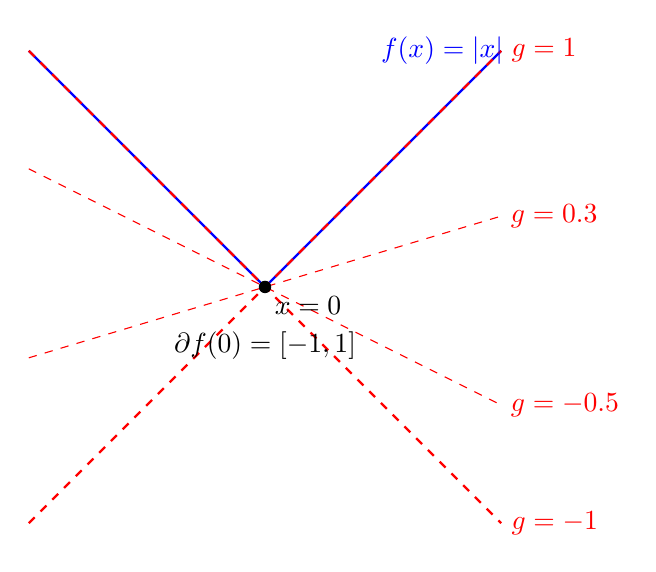
\begin{tikzpicture}[scale=1.5]
    % Function |x|
    \draw[thick, blue, domain=-2:0] plot (\x, {-\x});
    \draw[thick, blue, domain=0:2] plot (\x, {\x});

    % Subgradients at x=0
    \draw[red, dashed, domain=-2:2] plot (\x, {-0.5*\x}) node[right] {$g = -0.5$};
    \draw[red, dashed, domain=-2:2] plot (\x, {0.3*\x}) node[right] {$g = 0.3$};
    \draw[red, thick, dashed, domain=-2:2] plot (\x, {-\x}) node[right] {$g = -1$};
    \draw[red, thick, dashed, domain=-2:2] plot (\x, {\x}) node[right] {$g = 1$};

    \fill[black] (0,0) circle (1.5pt) node[below right] {$x = 0$};
    \node[blue] at (1.5, 2) {$f(x) = |x|$};
    \node at (0, -0.5) {$\partial f(0) = [-1, 1]$};
\end{tikzpicture}
\end{center}

\section{Python Implementation}

\begin{codeblock}[title=\textbf{Subgradient method for $\ell_1$ minimization}]
\begin{minted}{python}
import numpy as np
import matplotlib.pyplot as plt

def subgradient_l1(A, b, x0, n_iter=500, c=1.0):
    """Minimize ||Ax - b||_1 via subgradient method."""
    x = x0.copy()
    n = len(x)
    f_best = np.inf
    x_best = x.copy()
    history = []

    for k in range(n_iter):
        r = A @ x - b
        f_val = np.sum(np.abs(r))
        if f_val < f_best:
            f_best = f_val
            x_best = x.copy()
        history.append(f_best)

        # Subgradient of ||Ax - b||_1
        g = A.T @ np.sign(r)
        alpha = c / np.sqrt(k + 1)
        x = x - alpha * g

    return x_best, history

# Test
np.random.seed(42)
m, n = 50, 20
A = np.random.randn(m, n)
x_true = np.zeros(n)
x_true[:5] = np.random.randn(5)
b = A @ x_true + 0.1 * np.random.randn(m)

x0 = np.zeros(n)
x_sol, hist = subgradient_l1(A, b, x0, n_iter=1000)

plt.semilogy(hist)
plt.xlabel('Iteration')
plt.ylabel('Best f value')
plt.title('Subgradient method for L1 minimization')
plt.grid(True, alpha=0.3)
plt.savefig('subgradient_l1.pdf')
\end{minted}
\end{codeblock}

\section{Exercises}

\begin{exercise}[$\star$]
Compute the subdifferential of $f(x) = \max(0, x)$ at every point $x \in \R$.
\end{exercise}

\begin{exercise}[$\star$]
Compute $\partial f(x)$ for $f(x) = \norm{x}_2$ on $\R^n$.
\end{exercise}

\begin{exercise}[$\star\star$]
Let $f(x) = \max(x_1, x_2)$ on $\R^2$. Compute $\partial f(x)$ for $(x_1, x_2)$
with $x_1 > x_2$, $x_1 < x_2$, and $x_1 = x_2$.
\end{exercise}

\begin{exercise}[$\star\star$]
Prove the sum rule: if $f$ and $g$ are convex with
$\mathrm{dom}(f) \cap \mathrm{int}(\mathrm{dom}(g)) \neq \emptyset$, then
$\partial(f+g)(x) = \partial f(x) + \partial g(x)$.
\end{exercise}

\begin{exercise}[$\star\star$]
Show that the normal cone $N_C(x) = \partial \iota_C(x)$ is a closed convex cone.
\end{exercise}

\begin{exercise}[$\star\star\star$]
Show that $f$ is convex if and only if the operator $\partial f$ is monotone.
\end{exercise}

\begin{exercise}[$\star\star\star$]
Implement the subgradient method with Polyak step size to minimize
$f(x) = \norm{Ax - b}_1 + \lambda\norm{x}_\infty$ and compare with CVXPY.
\end{exercise}
